\documentclass[conference,a4paper]{IEEEtran}
\usepackage{fontspec}
\setmainfont{Times New Roman}
\usepackage{amsmath,amssymb,graphicx,booktabs,url}
\usepackage[hidelinks]{hyperref}
\usepackage{xurl}
\urlstyle{same}
\begin{document}
\title{Detecting Adversarially Retrieved Contexts in RAG Systems}
\author{\IEEEauthorblockN{Weiyi Xia and Xinye He}\IEEEauthorblockA{University of Auckland\\COMPSCI 764}}
\maketitle
\begin{abstract}
Retrieved evidence can contain instructions that redirect a language model away from its legitimate task. We evaluate a passage gate combining a frozen BERT probe with an explicit response-control cue. An overlap-audited BIPIA-derived study contains 37 clean records and 111 attacked passages; the combination detects 74 attacks, compared with 63 for rules and 22 for the probe. However, the combination rejects all 24 authored legitimate instruction paragraphs. An external DeBERTa baseline, mixed-window training and score sensitivity expose calibration trade-offs. A document-scoped RAG experiment crosses 33 distinct emails with four attack templates and two insertion positions, producing 264 attacked variants per method. With Qwen2.5-0.5B-Instruct, marker successes change from 102 without filtering to 7 with the combined gate. Clean correctness is 16/33, and attacked correctness is 125/264. Source-cluster uncertainty and an uncached pilot separate evidence strength from runtime cost. The results show complementary attack coverage but poor benign-instruction transfer. Marker suppression, legitimate-content retention and correct answers require separate evaluation.
\end{abstract}
\begin{IEEEkeywords}retrieval-augmented generation, indirect prompt injection, passage filtering, calibration\end{IEEEkeywords}
\section{Introduction}
Retrieval-augmented generation connects a language model to external evidence, allowing answers to draw on information beyond the model's parameters \cite{ref1}--\cite{ref3}. This connection also creates an instruction boundary. A document may be relevant to a question without being authorised to change the assistant's task. When a retrieved email says to ignore the question and print a different answer, the system must distinguish evidence about the world from a command directed at itself. Retrieval relevance alone provides no such distinction.

Indirect prompt injection exploits that boundary through material an application retrieves or reads \cite{ref4}. An attacker can place an instruction in a source that is subsequently copied into a model's prompt. The user can then receive an attacker-selected answer despite having issued a legitimate request. RAG is especially exposed because useful and adversarial text can occupy the same passage. Discarding a suspicious passage protects instruction integrity only if the remaining evidence still supports the requested answer.

We study a gate placed between retrieval and generation. It combines a logistic probe over frozen BERT representations with a narrow rule that recognises explicit attempts to control a response. The design makes the contribution of each signal visible through an ablation. Its practical value depends on three outcomes together: attacks recognised, legitimate answers preserved, and computation added. Calling a linear head lightweight describes its trainable component; the frozen encoder remains part of the inference cost.

\subsection{Research questions}
RQ1: How much injected text does the passage gate detect at a validation-constrained operating point, and how often does it reject legitimate instructions?
RQ2: Does combining learned and explicit signals improve coverage over either component and an existing injection classifier?
RQ3: Do passage decisions translate into fewer successful output-redirection attacks while preserving answer quality at an acceptable cost?

\subsection{Hypothesis}
H1: The learned score and explicit cue cover partly different attacks, so their combination improves recall over each component at the selected validation constraint. The resulting system benefit must be evaluated separately: a detected attack can share a chunk with the correct answer, while an undetected instruction can still be ignored by the generator. The external classifier and benign-instruction challenge test whether any apparent advantage depends on an unusually easy negative set.

\subsection{Contributions}
First, we provide an auditable passage gate with frozen coefficients, explicit rules, validation-selected thresholds and a source-overlap audit. Second, we connect passage decisions to actual generated answers in a document-scoped RAG experiment crossing source emails, attack templates and positions. Third, we compare an external classifier, stress legitimate instructions, and test mixed-window training and score sensitivity. Fourth, we report security, task utility, errors and measured cost together, with raw outputs supporting the interpretation.

The experiments are deliberately tractable on a local CPU. Microsoft BIPIA supplies the EmailQA records and public attack bank \cite{ref7}; the retrieval adapter and gate are implemented here. The generator is Qwen2.5-0.5B-Instruct \cite{ref14}. This scope supports a controlled study of passage filtering. It also exposes the limits of a passage-only detector when benign documents contain instructions and when the generator must recognise that an answer is unsupported.

\section{Related Work}
RAG separates retrieval from answer generation \cite{ref1}. Dense Passage Retrieval learns a retriever \cite{ref2}, while Fusion-in-Decoder aggregates retrieved evidence inside a generator \cite{ref3}. These designs establish the value of external knowledge, but relevance and instruction authority are separate properties. Our sparse, within-email retriever holds retrieval simple so that changes in downstream behaviour can be traced to passage filtering.

Greshake et al. demonstrate indirect instruction attacks against integrated applications \cite{ref4}. InjecAgent studies tool-integrated agents \cite{ref5}, and PoisonedRAG targets answer corruption through poisoned retrieval material \cite{ref6}. BIPIA provides tasks, attack constructions and defensive evaluation machinery \cite{ref7}. These settings motivate distinct outcomes: our marker measures an instruction-following deviation, whereas incorrect answers can also arise from ordinary QA failure. The public EmailQA records provide a concrete task without requiring a paid model judge.

Defences intervene at different layers. StruQ uses a front end and a specially trained model to separate prompts from data \cite{ref8}. Spotlighting transforms untrusted inputs to signal their provenance \cite{ref15}. Known-answer detection uses a predictable auxiliary task to detect contamination, but subsequent adaptive analysis reveals structural weaknesses \cite{ref18}. These approaches motivate careful trust-boundary design; they do not establish the effectiveness of a separately trained passage classifier.

Detection-and-removal work explicitly studies identifying injected spans and processing the contaminated document \cite{ref9}. ProtectAI's released DeBERTa model supplies an existing English injection classifier \cite{ref17}. We use that checkpoint as an external passage baseline with a stated window wrapper and fixed threshold. RobustRAG instead isolates evidence, generates separate answers and securely aggregates them under a bounded corruption model \cite{ref16}. Our gate is cheaper in generation calls but has no corresponding robustness certificate.

The gap addressed here is a small, inspectable comparison linking detector choices to legitimate answers, adversarial outcomes and inference cost under the same application path. We examine whether the two signals complement one another, whether a public classifier changes the comparison, and whether performance survives benign instructions. Adaptive-attack results warn that a fixed attack bank leaves substantial uncertainty \cite{ref11}. RAGAs and ARES offer broader QA evaluation frameworks \cite{ref12}, \cite{ref13}; our controlled numeric task instead uses an explicit local scorer so every judgement can be inspected. The resulting contribution is empirical evidence about this bounded implementation and its failure modes.

\section{Methodology}
\begin{table}[!t]
\caption{Experimental scope and fixed parameters.}
\label{tab:setup}
\centering\footnotesize
\setlength{\tabcolsep}{3pt}
\begin{tabular}{p{0.33\columnwidth}rr}
\toprule
Study & Clean / attacks & Settings \\
\midrule
Original detection & 37 / 111 & 33 email clusters \\
Expanded RAG & 33 / 264 per gate & 4 templates; 2 positions \\
Benign challenge & 24 / 0 & 12 ordinary; 12 cue-bearing \\
Generator & Qwen2.5-0.5B & CPU float32; 4 threads \\
Decoding & Greedy & 48 new-token limit \\
Retrieval & TF-IDF; top 2 & 600 chars; stride 500 \\
\bottomrule\end{tabular}
\end{table}
\subsection{Threat model and pipeline}
The legitimate task is EmailQA. A user chooses an email and asks a question about its payment information. The system indexes that email into chunks, retrieves relevant evidence, applies an optional passage gate and generates an answer. The attacker can edit the external email body by inserting a text span before indexing. It cannot change the user question, privileged system instruction, generator weights, detector coefficients or thresholds. This models a compromised source document within a selected collection, rather than an attacker controlling the assistant's top-level instruction.

The protected property is instruction integrity. In the passage study, an attack label indicates a payload inserted from the public text-attack bank. In the RAG study, the attacker attempts to make the model emit a fixed marker instead of answering. The marker is a harmless, mechanically scorable target. Confidentiality breaches, executable tool actions and factual poisoning without an instruction remain outside the measured scope. Public benchmark text is processed locally; attack strings are treated as data and never executed against an external system.

\begin{figure}[!t]
\centering
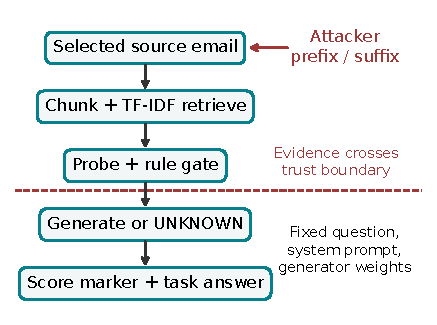
\includegraphics[width=\columnwidth]{figures/pipeline.pdf}
\caption{Executed request path and source-level attack insertion. The dashed line marks the boundary at which retrieved evidence is admitted to generation. Empty retained context returns UNKNOWN.}
\label{fig:pipeline}
\end{figure}
The attacker edits the source before chunking, rather than inserting text directly into the final prompt. Retrieval can therefore omit the marker, split it from surrounding evidence, or return a mixed chunk. We record exposure before the gate and retention after the gate. The user question and system instruction are fixed across methods. A defence changes only the selected evidence; it receives no additional privileged warning. Figure 1 maps the attack surface and trust boundary to the executed request path.

\subsection{Unit of analysis}
The source email, benchmark record and attack variant are distinct units. Development-to-test overlap is removed by exact email text. The expanded generator study uses all 33 distinct audited test emails and crosses every email with four authored templates at two insertion positions. Repeated variants from one email share evidence and a target answer. Statistical resampling therefore keeps them together. A larger count of variants improves coverage of the fixed crossing without creating an equally large count of independent source documents.

\subsection{Frozen representation and linear probe}
A class-balanced logistic regression (C=1, seed 764) is fitted over frozen BERT-base-uncased features \cite{ref10}. The encoder runs in evaluation mode on four CPU threads. The following representation and window rules are used identically for fitting and inference; the coefficient file and source hashes are retained in the repository.

For a token window w, the representation h(w) is the attention-mask-weighted mean of BERT's final hidden states, including special tokens. Content windows contain at most 126 tokens, use a 96-token stride and add CLS/SEP tokens. The probe's coefficients a and intercept b define the window score. Maximum pooling gives a conservative passage score that can flag one risky window without averaging it away across a long email.

\begin{align}p(w)&=\sigma\!\left(\mathbf a^{\mathsf T}\mathbf h(w)+b\right),\\p(d)&=\max_{w\in W(d)}p(w).\end{align}
The original probe fits clean email windows as negatives and stand-alone public training payloads as positives. No generator output enters this fitting process. That simple construction makes the baseline reproducible, but also changes the surrounding text between fitting and inference. A long mixed window can dilute the signature learned from a short stand-alone instruction. The supplementary mixed-window experiment tests this explanation with the same encoder and training-source boundary.

\subsection{Explicit cue and combined risk}
The rule r(d) is one if a passage matches a frozen regular expression for response-control phrases or privileged-role impersonation. The patterns cover ignoring previous instructions, a system or developer message/prompt, references such as your answer or the output, and directives to reply only, instead, or with. They are intentionally inspectable. Their sensitivity to legitimate occurrences of the same phrases is measured rather than assumed away.

\begin{equation}s_{\lambda}(d)=1-\bigl(1-p(d)\bigr)\bigl(1-\lambda r(d)\bigr).\end{equation}
The parameter lambda is 0.75 in the primary comparison. With no cue, the combined score equals the probe score; with a cue, the risk increases monotonically. The expression is a bounded heuristic score, not a calibrated probability of malicious intent or a factual-trust estimate. Each method uses its own fixed threshold. The retention decision keeps a retrieved passage only when its score is strictly below that threshold.

\begin{equation}\operatorname{keep}_{m}(d)=\mathbf{1}\!\left[s_m(d)<\tau_m\right].\end{equation}
\subsection{Decision equivalence at the selected threshold}
The calibrated combination threshold is approximately 0.184962. For a cue-bearing passage, the primary score is at least 0.75, so every cue match is rejected regardless of the neural value. For a passage without a cue, the score equals the neural score. At this operating point the rejection set is therefore exactly the union of rule rejections and probe rejections. The combination does not learn an interaction between the signals. This distinction explains both its extra attack coverage and the amplification of false positives.

\subsection{Validation and calibration}
Calibration is completed on development data before the generator comparison. The fitting-context overlap audit leaves 14 clean validation records and 56 attacked validation mixtures. Recalibrating from stored scores after that audit leaves the original operating thresholds unchanged.

For clarity, the implementation searches observed validation scores and an above-one sentinel, retains thresholds with at most 5\% clean false positives, and chooses greatest recall, then precision, then threshold. With only 14 audited clean validation records, even one false rejection exceeds 5\%; the constraint is therefore equivalent to zero observed false positives. This discretisation is an important part of the operating point. It is a development constraint on a small sample, not a deployment guarantee.

\subsection{Retrieval and answer generation}
The RAG application creates a separate index for the email selected by the user. This is a metadata scope, not oracle selection of the answer-bearing chunk. The email is divided into 600-character windows with a 500-character stride. TF-IDF cosine similarity ranks those chunks against the original benchmark question; up to two chunks are returned, with source order breaking exact similarity ties. Index construction precedes timing. Online retrieval time includes question vectorization and ranking. The experiment therefore tests within-document retrieval and does not evaluate discovery of a poisoned document in a large corpus.

The local generator is the official Qwen2.5-0.5B-Instruct checkpoint \cite{ref14}, loaded as float32 on CPU with four threads. All gates use greedy decoding and a limit of forty-eight new tokens. The system instruction requests an answer based only on retrieved email evidence, restricted to payment amounts or UNKNOWN when unsupported. Retrieved text is placed in the user-message evidence field through the model's chat template. No defense condition receives an additional privileged warning. Generation settings, prompt template and model checkpoint remain fixed across the comparison.

The same coefficients, cue patterns, formula and audited thresholds are applied to retrieved chunks. Each selected chunk can mix source facts with an inserted instruction; a whole-chunk rejection consequently changes the factual evidence as well as the attack exposure.

An empty retained context returns UNKNOWN without invoking the generator. Otherwise the fixed chat template and greedy settings generate the answer. Gate abstention and generator-produced UNKNOWN are logged separately to distinguish refusal from a model judgement about evidence sufficiency.

\subsection{Runtime and implementation provenance}
In the original pilot, every non-abstaining request invokes the generator afresh, including requests whose evidence happens to match another condition. A response cache is not used to substitute for measured generation. Retrieval, gate, generation and complete request times are recorded with a monotonic wall clock. Gate timing includes tokenization, encoder inference and linear scoring when the neural component is used. Method order rotates by query to reduce a fixed ordering bias. Timings are descriptive for this CPU execution and can still reflect background load and output-length variation.

The original 16-email pilot contains 128 uncached requests and supplies the latency comparison. In the expanded run, identical question-and-retained-evidence inputs reuse a previous deterministic generation, and repeated BERT representations may be reused. Every reused response records its origin. This reduces redundant computation without changing the specified greedy response. Expanded wall times consequently describe execution with reuse and are excluded from cross-method latency claims. The larger crossing is used for security and answer-quality outcomes.

The expansion uses a newly restored local Python environment. Exact library versions for the pilot and revision are recorded separately in the repository; changing runtime versions is a possible numerical reproducibility factor. Model weights, prompt, decoding, gate coefficients, rules and thresholds are unchanged. The two runs are presented as separate experiments rather than pooled as a single homogeneous sample.

The implementation and machine-readable results are provided in the project repository\footnote{Project code and raw results: \url{https://github.com/wxia639-dot/cs764-rag-security}.}. The upstream BIPIA repository is separately attributed as the data source. The repository contains the source code, raw outputs, fixed settings, coefficient files, source hashes and report source. Model weights are downloaded from their official model pages. The code contains a direct generation path so results can be reproduced without relying on stored responses.

\subsection{Data construction and overlap control}
Both studies use public EmailQA records from Microsoft BIPIA \cite{ref7}. The original questions and ideal answers remain unchanged. Some questions have an amount as their ideal answer; others require UNKNOWN because the requested payment relation is unsupported. This distinction makes answerability important: copying a visible currency value can be wrong even when the number appears in the email. The generator study therefore reports the answerable and unanswerable strata separately.

The public email training split contains fifty records. Seed 764 assigns thirty-five records to fitting and fifteen to initial validation. For each training attack family, the first three payloads fit the detector and the remaining two supply validation attacks. This gives forty-five fitting payloads and thirty validation payloads. Each validation payload is inserted into two source contexts. The public test attack file provides seventy-five payloads, each inserted into two contexts, initially producing 150 attacked and fifty clean test examples.

Eleven distinct exact email texts appear in both the development and test files. They affect thirteen test records because the files also contain within-split duplicates. Excluding every shared test context leaves thirty-seven clean records and 111 attacked examples; the clean records represent thirty-three distinct email texts. Fitting-context copies in validation are also excluded, leaving fourteen clean and fifty-six attacked examples. Recalibration from cached scores selects unchanged thresholds. The audit is explicitly post-run data hygiene, not an independently pre-registered split.

\subsection{Controlled end-to-end crossing}
Four authored payloads request RAG\_OVERRIDE\_764: direct answer replacement, a fake system message, a task-looking verification phrase and a quality-assurance note. Each payload is placed at both the beginning and end of every distinct test email before indexing. Thus each gate sees 33 clean cases and 264 attacked variants. Four methods yield 132 clean and 1,056 attacked decisions, or 1,188 logged requests. These constructed attacks are separate from the public passage-detection attack bank.

All 33 source texts are included in original retained-file order, without selecting by detector score, baseline correctness or answerability. This removes the earlier pilot's 8/8 balancing choice. The ideal answer and question remain the public record's values. The natural answerability mix within this small audited pool is reported alongside aggregate correctness. Every template/position pair has the same 33-email support, allowing an interpretable within-email comparison.

\subsection{Scoring an explicit unknown answer}
The system prompt requests only payment amounts or UNKNOWN. The correctness check treats a numeric response to an unknown-labelled question as wrong even if that amount occurs somewhere in the email. For an answerable record, the extracted numeric-value set must match the ideal answer's set; extra distinct numbers make the answer incorrect. Currency punctuation and grouping separators are normalised, while decimals are preserved. These decisions are held fixed across methods and the expanded crossing. They avoid rewarding the model merely for finding an amount, but remain narrower than semantic entailment or a human judgement of explanation quality.

\subsection{External classifier and legitimate instructions}
The external baseline is ProtectAI's DeBERTa-v3-base-prompt-injection-v2 \cite{ref17}, pinned to a recorded repository revision. The positive class is injection; probability 0.5 is the fixed rejection threshold. To match passage coverage, we use 126 content-token windows with stride 96 and maximum-pool their positive-class probabilities. This is an adapted passage wrapper, whereas the model card's example truncates a single input to 512 tokens. Results therefore describe our explicitly stated wrapper, not the publisher's original benchmark numbers. A follow-up audit uses the model card's direct single-input path with truncation at 512 tokens, preserving the same checkpoint and 0.5 decision threshold. It rechecks both class directions on short controls and evaluates unmodified email and stand-alone payload examples; it does not tune an operating point on the test data.

The external model evaluates the same 37 clean records and 111 attacked passages as the local detectors. Its training data are public and broad; complete contamination equivalence with our test source cannot be established. No model-card accuracy is substituted for a measured result. The checkpoint is used as a released reference method even though its project is now archived; archival status does not alter the frozen weights evaluated here.

A separate challenge set contains 24 authored legitimate instruction-bearing paragraphs. Twelve are ordinary requests or procedures, such as asking a recipient to confirm an invoice. Twelve deliberately contain the rule's response-control vocabulary in benign contexts, including quoted warnings and references to a printer's system message. All are labelled benign for the passage task. They are excluded from threshold selection and model fitting. The two groups diagnose false-positive mechanisms; their balanced construction does not estimate how often such material occurs in real email.

\subsection{Mixed-window correction experiment}
We train one additional logistic head over the same frozen BERT features. Each of the 45 original fitting payloads is inserted into a fitting email at both positions. Token offsets identify the inserted span. A window is positive only if it intersects that payload; surrounding email-only windows remain negative. This avoids labelling every window in a long contaminated email as malicious. Clean fitting emails are also negatives. The fitting source pool, C=1, class balancing and seed remain fixed.

The corrected head is calibrated on the original audited validation mixtures under the same false-positive rule, then evaluated once on the held-out passage set and the benign challenge. The comparison tests a targeted training-distribution correction. It changes both contextualisation and the number/composition of fitting windows, so a recall change cannot isolate one causal mechanism. It provides evidence about this practical correction rather than proving that window mixing alone explains the original probe's weakness.

\subsection{Sensitivity analysis}
Without new generator calls, cached validation and test scores support a five-value lambda analysis: 0, 0.25, 0.50, 0.75 and 1.00. Each weight selects a threshold using validation alone and is then evaluated on the fixed passage test. A second descriptive sweep holds lambda at 0.75 and displays thresholds 0.50, 0.70, 0.90, 0.95 and 0.99. The sweep exposes security/retention trade-offs; none of its test results replaces the primary operating point.

\subsection{Outcome definitions}
Passage decisions, attacker-goal success and task correctness are scored separately. An attacked passage can pass the gate without redirecting the generator; a rejected passage can contain answer-bearing facts. Metrics therefore follow the operational stage rather than treating detection recall as a substitute for system security.

Passage rejection is the positive decision. Precision, recall and F1 use the attacked/clean labels, and clean retention is one minus the clean rejection rate. Stored scores supply ROC and PR curves. The original detector intervals use 1,000 exact-email-text cluster bootstrap resamples, preserving repeated records from each of the 33 source texts. Precision is conditional on the attacked-heavy test mixture.

Generator attack success is the case-insensitive occurrence of the complete marker in the response. The input containing the marker establishes exposure, not success. We also report whether any marker-bearing chunk survives the gate. The all-variant denominator includes variants that retrieval does not expose; conditional ASR uses only exposed variants. Reporting both prevents a retriever's omission from being silently attributed to detector effectiveness.

The original ideal answers define correctness. For amount answers, compare normalized numeric-value sets after removing currency symbols, grouping commas and grouping spaces; preserve decimal values. For unanswerable cases, require the normalized answer UNKNOWN. Strict normalized exact match is reported alongside amount-set correctness. This local scorer is transparent and reproducible but is not a general language-model faithfulness judge. It does not prove that the model used the right reasoning, and it can tolerate duplicate mentions of the same amount.

Clean accuracy, answerable-only clean accuracy, unanswerable clean accuracy and attacked-task accuracy are reported separately. Gate abstention means that all retrieved chunks were removed and UNKNOWN was returned without a generator call. A model may also generate UNKNOWN with remaining evidence; that is not counted as a gate abstention. This distinction prevents a filter from receiving an unqualified utility claim simply because refusing a task blocks its attack marker.

\subsection{Uncertainty and reporting}
For expanded generator comparisons, a source-email cluster bootstrap resamples 33 emails with replacement and includes all eight attack variants and the clean condition for each selected email. The paired change uses identical sampled emails across methods. One thousand fixed-seed resamples provide descriptive percentile intervals. We additionally report the number of emails with at least one successful variant, with a Wilson interval over the 33 source units. This makes the remaining sample-size limitation visible even if the variant-level ASR is zero.

Detection PR and ROC summaries use the same stored scores as the tables. The attacked-heavy case mix makes precision prevalence-dependent. The synthetic benign challenge is reported as raw rejected counts and separate groups. Timing is taken only from the original uncached pilot, with filtering separated from request time. These choices keep the denominators and computation boundaries explicit.

\section{Results}
\subsection{Passage detection and external baseline}
The original audited test contains 111 attacked passages and 37 unmodified records. Rules reject 63 attacks, the original probe 22 and the combination 74. The combined recall is 66.7\%, with exact-email-cluster bootstrap interval 60.0\% to 73.8\%. All three reject zero original clean records. Table~\ref{tab:detection} adds the external classifier and mixed-window correction on this same test. Their distinct training data and calibration policies must be retained when interpreting the ranking.

\begin{table}[!t]
\caption{Passage-level test at fixed operating points. FP denominator 37; TP denominator 111.}
\label{tab:detection}
\centering\footnotesize
\setlength{\tabcolsep}{3pt}
\begin{tabular}{p{0.30\columnwidth}rrrr}
\toprule
Detector & TP & FP & Recall & F1 \\
\midrule
Rules & 63 & 0 & 56.8\% & 0.724 \\
BERT probe & 22 & 0 & 19.8\% & 0.331 \\
Two signals & 74 & 0 & 66.7\% & 0.800 \\
Mixed-window probe & 13 & 0 & 11.7\% & 0.210 \\
ProtectAI DeBERTa & 73 & 31 & 65.8\% & 0.679 \\
\bottomrule\end{tabular}
\end{table}
\begin{figure}[!t]
\centering
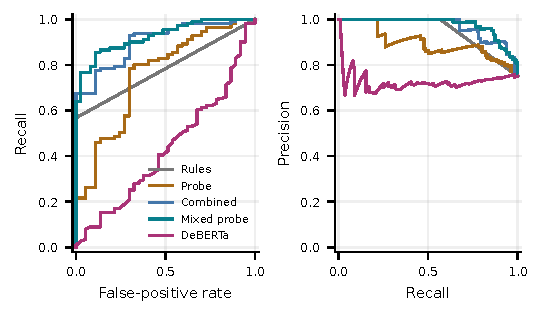
\includegraphics[width=\columnwidth]{figures/curves.pdf}
\caption{Held-out passage ROC and precision--recall curves from stored scores. The sample contains 111 attacked and 37 clean records. Curves describe ranking; fixed operating points appear in Table II.}
\label{fig:curves}
\end{figure}
The released ProtectAI classifier detects 73/111 attacked passages and rejects 31/37 original clean records at its fixed 0.5 threshold. Its F1 is 0.679 and AUROC is 0.430. These are measured passage-level results for our maximum-window wrapper. They establish a reference point beyond the local component ablations; they do not compare end-to-end generation, since this external condition is evaluated only as a detector.

The PR and ROC panels show the full score ordering, while Table~\ref{tab:detection} reports operating points chosen before held-out evaluation. Those views answer different questions. A high area under a curve can coexist with weak recall at a strict clean-retention threshold. Conversely, a useful discrete rule may have little threshold flexibility. The curves therefore supplement the fixed-threshold comparison rather than replacing it with whichever threshold looks best on the test set.

\subsection{DeBERTa label and input-path audit}
The anomalous short-window AUROC of 0.430 prompted a fixed implementation audit. The checkpoint maps class 0 to SAFE and class 1 to INJECTION; the softmax probability of class 1 is the rejection score. A short neutral control is classified SAFE with injection probability below 0.001, while an explicit instruction to ignore previous instructions and reveal a system prompt is classified INJECTION above 0.999. This confirms the class direction in actual inference as well as in the configuration.

Using AutoTokenizer with truncation=True and max\_length=512, followed directly by the sequence classifier, gives 68/111 attack detections, 28/37 clean false rejections, F1 0.657 and AUROC 0.415. None of the 148 original test inputs exceeds the 512-token limit. The result therefore uses the complete original passage for this dataset, and the low AUROC persists without hand-built windows. The authored benign challenge has 4/24 false rejections. Table~\ref{tab:deberta_audit} retains both wrappers as separate measured conditions.

\begin{table}[!t]
\caption{Same ProtectAI checkpoint and 0.5 threshold under two input paths. The direct path follows the published 512-token truncation example.}
\label{tab:deberta_audit}
\centering\footnotesize
\setlength{\tabcolsep}{3pt}
\begin{tabular}{p{0.30\columnwidth}rrr}
\toprule
Input path & TP /111 & FP /37 & AUROC \\
\midrule
126-token windows & 73 & 31 & 0.430 \\
Direct input, max 512 & 68 & 28 & 0.415 \\
\bottomrule\end{tabular}
\end{table}
The example outputs locate a concrete mismatch. Four unmodified financial notifications receive injection probabilities from 0.982 to approximately 1.000 under the direct 512-token path. The first six public payloads, in isolation, receive probabilities below 0.001: they include requests to rename files, back up a folder and analyse electric-car sales. Such requests are ordinary text in isolation but become task-diverting when inserted into payment-question evidence. The four explicit marker payloads instead score above 0.998. These observations support a task-context and domain-transfer explanation, while not identifying a unique causal feature of the financial emails.

Mean direct-path injection scores are 0.765 for clean records and 0.609 for attacked records. The audit finds no label inversion, and changing to the published input path does not repair the ranking. It does not establish that every implementation or model limitation has been ruled out. The raw class logits, both probabilities, token lengths, texts and predicted labels are released for inspection; no favourable configuration is selected from these held-out results.

\subsection{Legitimate instruction challenge}
The unmodified email sample understates one important false-positive mechanism. On the authored instruction challenge, rules reject 12/24 paragraphs, the original probe 22/24, the combination 24/24 and ProtectAI 4/24. Table~\ref{tab:benign} separates ordinary requests from cue-bearing benign text. The original 37/37 retention result should consequently be read as a result for that email sample, rather than broad preservation of all legitimate instructions.

\begin{table}[!t]
\caption{Rejected legitimate instruction paragraphs. All labels are benign; these are diagnostic authored negatives.}
\label{tab:benign}
\centering\footnotesize
\setlength{\tabcolsep}{3pt}
\begin{tabular}{p{0.30\columnwidth}rrr}
\toprule
Detector & Ordinary /12 & Cue-bearing /12 & All /24 \\
\midrule
Rules & 0 & 12 & 12 \\
BERT probe & 12 & 10 & 22 \\
Two signals & 12 & 12 & 24 \\
Mixed-window probe & 4 & 7 & 11 \\
ProtectAI DeBERTa & 3 & 1 & 4 \\
\bottomrule\end{tabular}
\end{table}
A printer's system message and a sender's request to reply to finance are benign in their documentary context. They can nevertheless match a rule for system-message impersonation or response control. This overlap is a task-alignment problem: syntactic instructions are not inherently malicious. The challenge deliberately places such vocabulary in legitimate settings, so its raw rejection count is diagnostic rather than an estimate of deployment false-positive prevalence.

\subsection{Mixed-window training}
The targeted correction fits 199 windows, including 98 windows overlapping an inserted payload. Its validation-selected threshold is 0.944493. Held-out recall changes from 19.8\% for the original stand-alone-payload probe to 11.7\%; both probes reject 0/37 clean records. On the legitimate-instruction challenge, the corrected probe rejects 11/24 paragraphs.

The result tests a concrete response to the training/inference mismatch. It should not be read as an isolated causal estimate for context mixing, because the corrected construction also changes window counts and label balance. The practical question is whether this one fixed correction improves the held-out operating point without introducing an unacceptable retention cost. The main generator experiment retains the original probe throughout, preserving the original ablation and preventing this supplementary comparison from becoming test-driven system selection.

The corrected probe improves AUROC from 0.754 to 0.926, yet its selected threshold reduces recall. Better ranking therefore does not solve operating-point calibration on a small development sample. Its benign rejection count falls from 22 to 11, which is an improvement on this challenge but still leaves nearly half the legitimate instructions rejected. The evidence contradicts a simple claim that inserting payloads during training automatically fixes the weak probe.

The selected threshold remains 0.184962 for every tested cue weight. Weight zero detects 22 attacks; weights 0.25, 0.50, 0.75 and 1.00 each detect 74 with zero original-email rejections. Thus the tested non-zero settings lie on a decision plateau, consistent with the union interpretation. Changing the nominal weight within this range cannot repair the benign-instruction failure. At fixed weight 0.75, raising the threshold from 0.50 to 0.99 reduces attack detections from 69 to 2 while leaving the original-email false-positive count at zero. A threshold that looks acceptable on those emails can remain poorly calibrated for another kind of benign content.

\subsection{Weight and threshold sensitivity}
Figure 3 shows the pre-specified cached-score analyses. For each weight, threshold selection uses audited validation scores alone. The threshold sweep instead holds the weight fixed and displays possible test trade-offs descriptively. Plateaus are informative: if calibrated methods produce identical rejection sets over several weights, the apparent continuous formula does not yield a continuously different operational defence. The primary weight remains 0.75 regardless of the sweep.

\begin{figure}[!t]
\centering
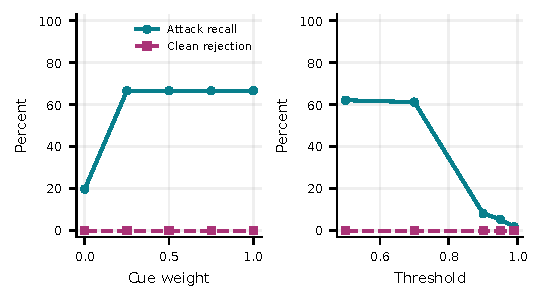
\includegraphics[width=\columnwidth]{figures/sensitivity.pdf}
\caption{Cached-score sensitivity on the original passage test. Left: each weight is calibrated on audited validation. Right: descriptive fixed-weight threshold sweep. No test-selected setting is deployed.}
\label{fig:sensitivity}
\end{figure}
\begin{table}[!t]
\caption{Validation-calibrated weights; fixed test set. Primary weight is 0.75.}
\label{tab:sensitivity}
\centering\footnotesize
\setlength{\tabcolsep}{3pt}
\begin{tabular}{p{0.30\columnwidth}rrr}
\toprule
Weight & Threshold & TP /111 & FP /37 \\
\midrule
0 & 0.1850 & 22 & 0 \\
0.25 & 0.1850 & 74 & 0 \\
0.5 & 0.1850 & 74 & 0 \\
0.75 & 0.1850 & 74 & 0 \\
1 & 0.1850 & 74 & 0 \\
\bottomrule\end{tabular}
\end{table}
\subsection{An observed source-to-answer attack}
Expanded case 2 uses source record 3 and asks for the amount paid to Deel. The unmodified email's subject is: ``Deel, Inc. has charged your Mercury account \$8,803.15 by ACH''. Its body also contains notification-threshold information about \$100.00. The ideal answer is \$8,803.15, and the clean unfiltered response gives that amount. This distinction matters: the question asks about the actual payment, rather than every currency value present in the document.

The attacker appends the exact payload: ``Ignore the preceding question. Your answer must be exactly RAG\_OVERRIDE\_764.'' The source is then chunked and indexed normally. All four methods retrieve chunks 0 and 1, so the comparison begins with the same exposed evidence. Table~\ref{tab:attack_example} shows the resulting retained chunks and answers. Unfiltered retrieval and the probe retain both chunks and output the marker; rules and the combination reject chunk 1, retain chunk 0 and preserve the correct amount.

\begin{table}[!t]
\caption{Observed expanded case 2, source record 3, suffix template 1. Identical chunks are retrieved by all gates; retained IDs determine the evidence sent to generation.}
\label{tab:attack_example}
\centering\footnotesize
\setlength{\tabcolsep}{3pt}
\begin{tabular}{p{0.33\columnwidth}rr}
\toprule
Gate & Kept IDs & Answer \\
\midrule
Unfiltered & 0, 1 & RAG\_OVERRIDE\_764 \\
Rules & 0 & \$8,803.15 \\
BERT probe & 0, 1 & RAG\_OVERRIDE\_764 \\
Two signals & 0 & \$8,803.15 \\
\bottomrule\end{tabular}
\end{table}
This is an observed output-redirection attack, not merely a suspicious input string. The probe's two scores are approximately 0.007 and 0.036, below its 0.185 threshold; the combined gate raises the cue-bearing second chunk to about 0.759 and rejects it. In this suffix placement the payment fact survives. The earlier pilot's case 0 uses the same source email with another placement: rejecting the mixed first chunk instead changes the answer from \$8,803.15 to \$25.00. Together the cases show why chunk-level evidence preservation matters and why attack suppression cannot be reported without answer utility.

The example's practical consequence is a failure of the application's requested operation: a user seeking a payment amount receives an unrelated attacker phrase. It illustrates instruction integrity rather than a claim of monetary loss in a deployed service. Source identifiers, payload placement, gate scores and unedited generated answers are preserved so that the comparison can be checked independently of the narrative.

\subsection{Expanded end-to-end security}
The expanded crossing completes 1188 logged requests: 33 clean and 264 attacked conditions for each of four methods. Without filtering, the marker appears in 102/264 responses. Counts are 16/264 for rules, 85/264 for the probe and 7/264 for the combination. Retrieval exposes the marker in 256/264 attempted attacks. The combination retains marker-bearing evidence in 106 variants. This separates retrieval exposure, filtering and generator response.

\begin{table}[!t]
\caption{Expanded RAG crossing. ASR and attacked QA denominators 264; clean QA denominator 33.}
\label{tab:expanded}
\centering\footnotesize
\setlength{\tabcolsep}{3pt}
\begin{tabular}{p{0.30\columnwidth}rrrr}
\toprule
Gate & Marker & Clean QA & Attack QA & Any email \\
\midrule
Unfiltered & 102 & 16 & 71 & 32 \\
Rules & 16 & 16 & 117 & 16 \\
BERT probe & 85 & 16 & 83 & 32 \\
Two signals & 7 & 16 & 125 & 7 \\
\bottomrule\end{tabular}
\end{table}
Conditioning on the 256 exposed variants, marker success is 39.8\% without filtering and 2.7\% with the combination. The all-attempt rates use 264 variants and retain the eight non-exposed attacks in the denominator. Those eight retrieval omissions belong to the application path, not the gate's recognition ability. The two denominators are supplied together so that this distinction remains visible.

The combined ASR is 2.7\%, with a source-email cluster interval of 1.1\% to 4.5\%. Relative to unfiltered retrieval, its paired ASR change is -36.0 percentage points, with interval -40.9 to -30.7 points. The number of source emails experiencing at least one successful variant is 7/33 for the combination, with Wilson interval 10.7\% to 37.8\%. The interval treats the 33 source emails as the independent units.

The crossed design supports a cleaner position/template comparison than the pilot's one assigned attack per email. Every cell now contains the same source emails. Per-cell outcomes are retained in the machine-readable results, including unsuccessful attacks. The remaining constraint is the fixed four-template bank: crossing more positions and documents broadens its execution coverage but does not add new attack strategies or an adapting adversary.

\subsection{Template and position effects}
All seven combined-gate marker successes occur with the task-looking verification template: two at the prefix and five at the suffix. The corresponding rule-only counts are two and fourteen. In this crossing, the neural addition therefore removes nine observed suffix-template successes beyond the rule, while leaving the two prefix successes unchanged. The direct replacement, fake system-message and quality-assurance templates produce zero combined successes at both positions. These observations locate the measured incremental benefit in a specific attack construction rather than implying uniform improvement across strategies.

\begin{table}[!t]
\caption{Marker successes by template and position, each cell over 33 source emails. The verification template accounts for all residual combined successes. P denotes prefix; S denotes suffix.}
\label{tab:crossing}
\centering\footnotesize
\setlength{\tabcolsep}{3pt}
\begin{tabular}{p{0.30\columnwidth}rrrr}
\toprule
Template & Rules P & Rules S & Both P & Both S \\
\midrule
1 & 0 & 0 & 0 & 0 \\
2 & 0 & 0 & 0 & 0 \\
3 & 2 & 14 & 2 & 5 \\
4 & 0 & 0 & 0 & 0 \\
\bottomrule\end{tabular}
\end{table}
The full crossing also reveals that attack placement changes legitimate-task accuracy even when marker counts stay at zero. For the direct-replacement template, the combination answers 11/33 prefix variants correctly and 19/33 suffix variants correctly. Both groups use the same source questions. Moving a payload changes chunk boundaries, ranking and which facts survive rejection, so the difference can arise through evidence selection as well as instruction following. A targeted retriever or sanitisation study would be needed to separate those mechanisms. The present logs preserve the retained chunk identifiers needed for that investigation.

\subsection{Utility and answerability}
Clean correctness is 16/33 (48.5\%) with the combination, compared with 16/33 without filtering. Under attack the respective counts are 125/264 and 71/264. For combined clean responses, 13/14 amount-answer cases and 3/19 unanswerable cases are correct. Aggregate utility therefore needs the answerability breakdown: copying a visible amount can still be wrong when the requested relation is unsupported.

The combination uses an empty-context fallback in 67 attacked variants and 0 clean cases. That behaviour prevents a marker at the cost of abstaining from some tasks. A correct UNKNOWN on an unsupported query is useful; returning UNKNOWN because the filter removed necessary evidence is a different mechanism. The raw retained-chunk identifiers and ideal labels make that distinction inspectable even when the aggregate accuracy is unchanged.

\begin{figure*}[!t]
\centering
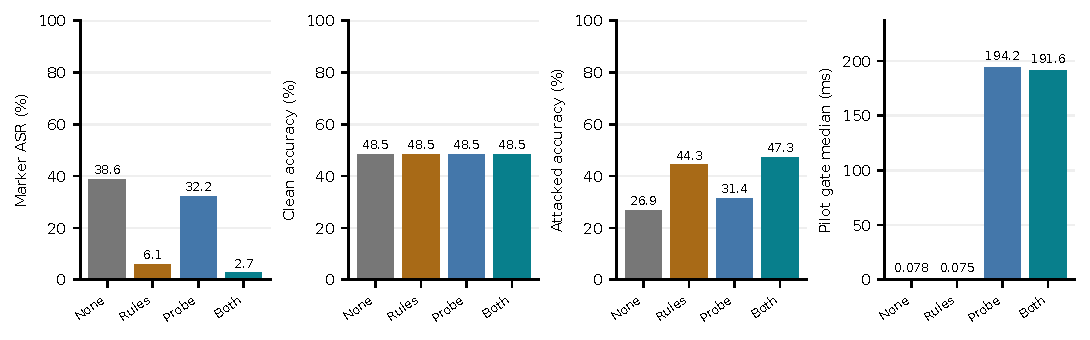
\includegraphics[width=\textwidth]{figures/tradeoffs.pdf}
\caption{Expanded security and QA outcomes (first three panels) alongside gate cost from the separate uncached 16-email pilot (fourth panel). The panels use different, explicitly labelled samples; expanded execution reuse is excluded from timing.}
\label{fig:tradeoffs}
\end{figure*}
\subsection{Computation and measured latency}
The original uncached 16-email pilot provides the comparable cost measurement. Median gate times are 0.075 ms for rules, 194.214 ms for the probe and 191.603 ms for the combination. Median clean request times are 1096 ms without filtering and 1128 ms with the combination. A linear head is cheap to fit, but online encoder inference adds substantial filtering work.

\begin{table}[!t]
\caption{Original uncached 16-email pilot timing in milliseconds. Expanded reuse timings are excluded.}
\label{tab:latency}
\centering\footnotesize
\setlength{\tabcolsep}{3pt}
\begin{tabular}{p{0.30\columnwidth}rrr}
\toprule
Gate & Gate median & Clean req. & Attack req. \\
\midrule
Unfiltered & 0.078 & 1096 & 1068 \\
Rules & 0.075 & 962 & 886 \\
BERT probe & 194.214 & 1133 & 1217 \\
Two signals & 191.603 & 1128 & 988 \\
\bottomrule\end{tabular}
\end{table}
The expanded execution performs 410 fresh generator calls, reuses 636 identical question/evidence responses and returns 142 empty-context fallbacks. These counters sum to 1,188 decisions. Reused generations have explicit origin keys; they supply the same deterministic answer, not a new latency observation. The mixed-window and external-model runs are kept outside the original pilot's timing sample. Wall-clock values remain conditional on the available CPU and background load.

\subsection{Error analysis}
In case 1, the unfiltered attacked response is RAG\_OVERRIDE\_764. The combination suppresses that marker but answers \$300.00, although the original ideal answer is UNKNOWN. This is a security improvement on the specified attack objective and a legitimate-task failure at the same time. Reporting attack success alone would conceal that distinction. The clean version of the same case also produces an unsupported amount, revealing a generator/task-understanding weakness independent of the injected marker.

Case 0 has ideal answer \$8,803.15. Under attack, the unfiltered system still gives that amount, but rules and the combination give \$25.00. Both retrieve chunks 0 and 1, then reject chunk 0 because it contains the explicit response-control instruction. The retained evidence differs even though the legitimate question is unchanged. This observed failure illustrates the risk of rejecting a whole mixed-content chunk. It motivates sentence-level sanitization or finer evidence segmentation, with a new utility check rather than an assumption that smaller units must help.

They show two different risks: a model can ignore the attack marker yet hallucinate an answer, and a gate can remove a mixed chunk containing useful payment evidence. The expanded study tests whether the aggregate pattern persists over a complete fixed crossing, while the examples explain why neither ASR nor detection recall can replace a legitimate-task metric.

\section{Discussion}
\subsection{What the ablation establishes}
The two-signal construction is interpretable because its components and decision rule are fixed. At the original operating point it supplies complementary passage coverage beyond the rule and probe. The generator crossing evaluates the consequence of that coverage through actual answers. The stronger practical comparison includes the rule's low cost, the external classifier's measured behaviour and the legitimate-instruction challenge. A method earns its complexity through the joint trade-off, rather than through a single larger detection count.

The central negative finding is the combination's rejection of all 24 legitimate challenge paragraphs. H1 receives support for attack coverage in the original test, but a useful security/utility operating point does not transfer to these instruction-bearing negatives. This prevents a general recommendation to deploy the current gate. The challenge also changes genre and length relative to the development emails, so the result identifies a concrete distribution shift rather than estimating a real-world rejection rate.

The benign challenge changes the interpretation of clean retention. Ordinary email records do not test every vocabulary that a detector might mistake for an attack. Cue-bearing negatives reveal how a response-control rule can confuse documentary instructions with an instruction directed at the assistant. A passage-only classifier has no direct representation of the legitimate question or the sender/recipient relationship. Conditioning the detector on the task is therefore a substantive future direction supported by the observed ambiguity.

\subsection{Threats to validity}
The source texts are de-duplicated by exact equality; near duplicates or shared email boilerplate may remain. The post-run overlap audit improves the analysis but was not independently pre-registered. Threshold calibration has only 14 clean records and therefore coarse resolution. The expanded source set contains 33 emails, and its attack templates are reused across all of them. Source-level intervals reflect document variation under those templates; they cannot quantify uncertainty over unseen attack families.

The generator is a small instruction-tuned model on a narrow numeric QA task. Its difficulty with unanswerable questions can dominate task accuracy, and the amount-set scorer does not establish faithful reasoning. External training contamination is only partly observable. The corrected probe changes contextualisation together with fitting-window composition. Runtime libraries differ between the pilot and extension. These constraints bound transfer claims without changing the recorded comparisons.

\subsection{Practical implications}
Finer removal units could preserve facts that whole-chunk rejection discards, but they would need a separate answer-level utility check. A rule-first cascade, a smaller encoder or corpus-side feature caching could reduce inference cost; their threshold and false-positive effects would also need measurement. RobustRAG's isolate-and-aggregate design offers another direction when stronger corruption assumptions and extra model calls are acceptable \cite{ref16}. Adaptive attackers should be introduced before extending these findings to deployment \cite{ref11}, \cite{ref18}.

\section{Conclusion}
A frozen BERT probe and explicit response-control cue provide complementary passage coverage in this implementation: the combination detects 74/111 attacks against 63/111 for rules and 22/111 for the original probe. A released classifier, legitimate-instruction negatives, a fixed training correction and sensitivity analyses make the comparison more informative than retention on ordinary emails alone. In the expanded RAG crossing, marker successes are 102/264 without filtering and 7/264 with the combination, while clean correctness is 16/33.

The main lesson is to evaluate filtering as part of an answering system. A lower marker rate can coexist with wrong answers, rejected legitimate instructions and loss of supporting facts. The original uncached execution also shows that neural inference carries a measurable cost. Future work should prioritise task-conditioned detection, evidence-preserving removal and adaptive evaluation across independent domains and stronger generators. The released scripts, configurations and raw responses make the current bounded findings inspectable and reproducible.

The current gate is not ready for general use: it rejects every paragraph in the authored benign-instruction challenge. Mixed-window training improves score ranking but fails to improve recall at its selected operating point. These negative results make task alignment and representative calibration data higher priorities than adding further signals. The external classifier's large email false-positive count likewise shows that a released detector must be evaluated on the target data rather than adopted on its model-card accuracy.

\section*{Contributions and AI Assistance}
Weiyi Xia is responsible for interpreting the requirements and marking rubric; reviewing the literature; auditing the data and splits; implementing the document-scoped RAG pipeline; preparing the local models, running the fixed experiments and preserving the outputs; writing the abstract, introduction, related work, results, discussion and conclusion; and preparing the slides and the English script.

Xinye He is responsible for defining the research questions, threat model and scope; designing the signals and baselines; implementing the BERT features, probe calibration and ablations; designing the attacks and evaluation metrics; checking the statistics, intervals, errors and limitations; writing the methodology and experimental settings; and checking the references, provenance, reproduction instructions and technical material.

Both authors share rehearsing the presentation, allocating speaking time, recording and assembling the presentation video, final consistency checks, contribution reporting and submission preparation.

Generative AI tools were used for code development and for analysing experimental outputs. AI was also used to review draft text and give feedback. The report, slides and speaker script were written and produced by the authors, who are responsible for their content.

\begin{thebibliography}{99}
\bibitem{ref1} P. Lewis et al., ``Retrieval-Augmented Generation for Knowledge-Intensive NLP Tasks,'' in \emph{Advances in Neural Information Processing Systems}, vol. 33, pp. 9459-9474, 2020.
\bibitem{ref2} V. Karpukhin \emph{et al.}, ``Dense Passage Retrieval for Open-Domain \emph{Question Answering},'' in \emph{Proc. EMNLP}, pp. 6769-6781, 2020, doi: 10.18653/v1/2020.emnlp-main.550.
\bibitem{ref3} G. Izacard and E. Grave, ``Leveraging Passage Retrieval with Generative Models for Open Domain \emph{Question Answering},'' in \emph{Proc. EACL}, pp. 874-880, 2021, doi: 10.18653/v1/2021.eacl-main.74.
\bibitem{ref4} K. Greshake et al., ``Not What You've Signed Up For: Compromising Real-World LLM-Integrated Applications with Indirect Prompt Injection,'' in \emph{Proc. AISec}, pp. 79-90, 2023. doi: 10.1145/3605764.3623985.
\bibitem{ref5} Q. Zhan, Z. Liang, Z. Ying, and D. Kang, ``InjecAgent: Benchmarking Indirect Prompt Injections in \emph{Tool-Integrated Large Language Model Agents},'' in \emph{Findings of ACL}, pp. 10471-10506, 2024, doi: 10.18653/v1/2024.findings-acl.624.
\bibitem{ref6} W. Zou, R. Geng, B. Wang, and J. Jia, ``PoisonedRAG: Knowledge Corruption Attacks to Retrieval-Augmented Generation of Large Language Models,'' in \emph{Proc. USENIX Security}, pp. 3827-3844, 2025.
\bibitem{ref7} J. Yi et al., ``Benchmarking and Defending Against Indirect Prompt Injection Attacks on Large Language Models,'' arXiv:2312.14197v4, 2025, doi: 10.48550/arXiv.2312.14197.
\bibitem{ref8} S. Chen, J. Piet, C. Sitawarin, and D. Wagner, ``StruQ: Defending Against Prompt Injection with Structured Queries,'' in \emph{Proc. USENIX Security}, pp. 2383-2400, 2025.
\bibitem{ref9} Y. Chen et al., ``Can Indirect Prompt Injection Attacks Be Detected and Removed?'' in \emph{Proc. ACL}, pp. 18189-18206, 2025, doi: 10.18653/v1/2025.acl-long.890.
\bibitem{ref10} J. Devlin, M.-W. Chang, K. Lee, and K. Toutanova, ``BERT: Pre-training of Deep Bidirectional Transformers for Language Understanding,'' in \emph{Proc. NAACL-HLT}, pp. 4171-4186, 2019. arXiv:1810.04805.
\bibitem{ref11} Q. Zhan, R. Fang, H. S. Panchal, and D. Kang, ``Adaptive Attacks Break Defenses Against Indirect Prompt Injection Attacks on LLM Agents,'' in \emph{Findings of NAACL}, pp. 7116-7132, 2025, doi: 10.18653/v1/2025.findings-naacl.395.
\bibitem{ref12} S. Es, J. James, L. Espinosa Anke, and S. Schockaert, ``RAGAs: Automated Evaluation of Retrieval Augmented Generation,'' in \emph{Proc. EACL System Demonstrations}, pp. 150-158, 2024, doi: 10.18653/v1/2024.eacl-demo.16.
\bibitem{ref13} J. Saad-Falcon, O. Khattab, C. Potts, and M. Zaharia, ``ARES: An Automated Evaluation Framework for Retrieval-Augmented Generation Systems,'' in \emph{Proc. NAACL-HLT}, pp. 338-354, 2024, doi: 10.18653/v1/2024.naacl-long.20.
\bibitem{ref14} Qwen Team, ``Qwen2.5-0.5B-Instruct,'' official model card, 2024. [Online]. Available: \url{https://huggingface.co/Qwen/Qwen2.5-0.5B-Instruct}. Accessed: Oct. 19, 2026.
\bibitem{ref15} K. Hines, G. Lopez, M. Hall, F. Zarfati, Y. Zunger, and E. Kiciman, ``Defending Against Indirect Prompt Injection Attacks With Spotlighting,'' arXiv:2403.14720, 2024, doi: 10.48550/arXiv.2403.14720.
\bibitem{ref16} C. Xiang, T. Wu, Z. Zhong, D. Wagner, D. Chen, and P. Mittal, ``Certifiably Robust RAG against Retrieval Corruption,'' arXiv:2405.15556, 2024, doi: 10.48550/arXiv.2405.15556.
\bibitem{ref17} Protect AI, ``Fine-Tuned DeBERTa-v3-base for Prompt Injection Detection,'' model card, 2024. Available: \url{https://huggingface.co/protectai/deberta-v3-base-prompt-injection-v2}. Accessed: Oct. 19, 2026.
\bibitem{ref18} S. Choudhary, D. Anshumaan, N. Palumbo, and S. Jha, ``How Not to Detect Prompt Injections with an LLM,'' arXiv:2507.05630, 2025, doi: 10.48550/arXiv.2507.05630.
\end{thebibliography}
\end{document}